% SVN info for this file
\svnidlong
{$HeadURL$}
{$LastChangedDate$}
{$LastChangedRevision$}
{$LastChangedBy$}

\chapter{Working With BMI}
\labelChapter{Chapter_2}

\begin{introduction}
  This chapter will guide through the steps of working with BMI.
\end{introduction}

\section{Core Commands in BMI}

We will explore the following six commands in BMI: \\

\begin{itemize}
\item[\index{bmi pro}\code{pro }$\blacktriangleright$\hspace{-12mm}] \hspace{10mm}\emph{Provisions a node.}
\item[\index{bmi dpro}\code{dpro }$\blacktriangleright$\hspace{-12mm}] \hspace{10mm}\emph{Deprovisions a node.}
\item[\index{bmi snap}\code{snap }$\blacktriangleright$\hspace{-12mm}] \hspace{10mm}\emph{Takes a snapshot of a node.}
\item[\index{bmi ls}\code{ls }$\blacktriangleright$\hspace{-12mm}] \hspace{10mm}\emph{Lists store images.}
\item[\index{bmi ls}\code{import }$\blacktriangleright$\hspace{-12mm}] \hspace{10mm}\emph{Importing images or snapshots into BMI for provisioining.}
\item[\index{bmi db}\code{db }$\blacktriangleright$\hspace{-12mm}] \hspace{10mm}\emph{Database commands that about imported images or snapshots.} \\
\end{itemize}

Using these commands we will run through the end-to-end workflow shown in Figure \ref{fig:bmi-workflow-end-to-end}. 


%\pagebreak

\begin{figure}[!h] % Example of including images
\vspace{10mm}
\label{fig:bmi-workflow-end-to-end}
\begin{center}
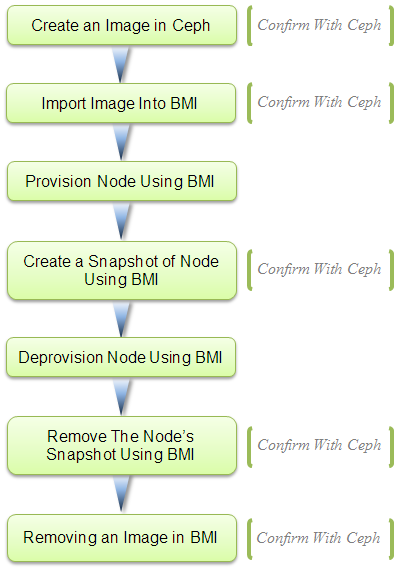
\includegraphics[scale=1.2]{figures/bmi-workflow-with-image-cleanup-v2.png}
\end{center}
\caption{HIL and BMI Ecosystem}
%\label{fig:example_figure}
\end{figure}


\section{Creating a Mock HIL and BMI Ecosystem}


In order to better learn how to use BMI, we will need to setup the a Ceph storage location, HIL and BMI instance.  The first step is to ensure that one has either a RedHat Enterprise Linux or Ubuntu instance with at least 5 GB of available storage with \code{sudo} access.  This can be performed via a virtual machine (VM).  Once that is created and you booted into the machine, you will need to \code{git-clone} the setup scripts, via the steps provided on the following page.

\pagebreak

\code{
\text{}\vspace{-10mm} \\
\text{}\hspace{6mm} git clone https://github.com/CCI-MOC/ims.git \\
\text{}\hspace{6mm} cd ims \\
\text{}\hspace{6mm} git fetch origin pull/60/head:pr-60 \\
\text{}\hspace{6mm} git checkout pr-60 \\
}

This will ensure that you have the proper install scripts and codebase to install Ceph, HIL and BMI.

\pagebreak

\subsection{Installing Ceph, HIL and BMI}

First it is important to prepare the environment for installation.  It is recommended you use either CentOS or Ubuntu (preferred) for your installation.  Each of these might require one to perform these commands: \\

\underline{\emph{For Ubuntu}} 

\code{
\text{} \\
\text{}\hspace{6mm} sudo add-apt-repository -y ppa:fkrull/deadsnakes \\
\text{}\hspace{6mm} sudo apt-get -y update \\
\text{}\hspace{6mm} sudo apt-get -y install python2.7 \\
\text{}\hspace{6mm} sudo ln -s /usr/bin/python2.7 /usr/bin/python \\
}

\underline{\emph{For CentOS}} 

\code{
\text{} \\
\text{}\hspace{6mm} sudo yum -y install git \\
}

Next you will need to prepare the Ceph configuration file by going to the install directory, as follows:

%In order to install type the following at the Bash prompt: 


\code{
\text{} \\
\text{}\hspace{6mm} cd scripts/install/ \\
%\text{}\hspace{6mm} ./install.sh \\
}

And subsequently running the following Ceph configuration script:


\code{
\text{} \\
\text{}\hspace{6mm} \small\#!/bin/bash \\
\text{}\hspace{6mm} if [ ! -z  "`sudo ls /etc/ | grep redhat-release`" ]; then \\
\text{}\hspace{12mm}   cp /etc/hostname . \\
\text{}\hspace{12mm}   cat /etc/hostname | cut -f1 -d'.' > hostname \\
\text{}\hspace{12mm}   sudo cp hostname /etc \\
\text{}\hspace{6mm} fi \\
\text{}\hspace{6mm} if [ ! -z "`ifconfig | grep inet | head -n1 | grep :`" ]; then \\
\text{}\hspace{12mm}   IP\_ADDRESS=`ifconfig | grep inet | head -n1 | cut -f2 -d':' | cut -f1 -d' '` \\
\text{}\hspace{6mm} else \\
\text{}\hspace{12mm}   IP\_ADDRESS=`ifconfig | grep inet | head -n1 | cut -f2 -d'i' | cut -f2 -d' '` \\
\text{}\hspace{6mm} fi \\
\text{}\hspace{6mm} echo -e "public\_network = \$IP\_ADDRESS/24\textbackslash{}nosd pool default size = 2\textbackslash{}nosd crush chooseleaf type = 0" >{}> ceph.conf \\
}

At this point you can initiate the installation process as follows:

\code{
\text{} \\
%\text{}\hspace{6mm} cd scripts/install/ \\
\text{}\hspace{6mm} ./install.sh \\
}

\pagebreak

After the installation first check that \index{Ceph}Ceph is operational:

\code{
\text{} \\
\text{}\hspace{6mm} ceph -s \\
}

You should see the following, which should be indicated by \code{HEALTH\_OK} under the \emph{health} attribute:

\code{
\text{} \\
\text{}\hspace{6mm} cluster 2469e0b1-9269-434a-8dc5-047c863f70e0 \\
\text{}\hspace{6mm} health HEALTH\_OK \\
\text{}\hspace{6mm} monmap e1: 1 mons at {pgrosu-pr-60=192.168.1.14:6789/0} \\
\text{}\hspace{12mm} election epoch 3, quorum 0 pgrosu-pr-60 \\
\text{}\hspace{6mm} osdmap e31: 3 osds: 3 up, 3 in \\
\text{}\hspace{12mm} flags sortbitwise,require\_jewel\_osds \\
\text{}\hspace{6mm} pgmap v87: 112 pgs, 7 pools, 19066 kB data, 184 objects \\
\text{}\hspace{12mm} 140 MB used, 14466 MB / 14606 MB avail \\
\text{}\hspace{22mm} 112 active+clean \\
}

Next check the \index{Ceph}Ceph version via the following command: 

\code{
\text{} \\
\text{}\hspace{6mm}  ceph --version \\
}

You should see the following output: 

\code{
\text{} \\
\text{}\hspace{6mm} ceph version 10.2.7 (50e863e0f4bc8f4b9e31156de690d765af245185) \\
}

Next check the \index{ceph-deploy}\code{ceph-deploy} version via the following command: 

\code{
\text{} \\
\text{}\hspace{6mm} ceph-deploy --version \\
}

You should see the following output: 

\code{
\text{} \\
\text{}\hspace{6mm} 1.5.38 \\
}

Next check that \index{RBD}RBD is operational via the following command: 

\code{\text{} \\
\text{}\hspace{6mm} rbd ls \\
}

\pagebreak

You should see the following listed images: 

\code{
\text{} \\
\text{}\hspace{6mm} 112233445566778899img1 \\
\text{}\hspace{6mm} cirros-0.3.0-x86\_64-disk.img \\
}

%\pagebreak

Next you will need to set the HIL \emph{username} and \emph{password} that is in the \code{bmi\_userrc.sh} file, by typing the following command:

\code{
\text{} \\
\text{}\hspace{6mm} source bmi\_userrc.sh \\
}

That file just contains the following two entries: 

%\pagebreak 

\code{
\text{} \\
\text{}\hspace{6mm} export HAAS\_USERNAME=haas \\
\text{}\hspace{6mm} export HAAS\_PASSWORD=secret \\
}

Next we can enter the BMI virtual environment via the following two commands: 

\code{
\text{} \\
\text{}\hspace{6mm} cd $\sim$/ims/ \\
\text{}\hspace{6mm} source .bmi\_venv/bin/activate \\
}

You will know that you are in the virtual environment if you see the prompt being prefixed by \code{(.bmi\_venv)} displayed as follows: 

\code{
\text{} \\
\text{}\hspace{6mm} (.bmi\_venv) ubuntu@pgrosu-pr-60:$\sim$/ims\$ \\
} 

The Einstein and Picasso servers are already running, which you can verify by the following command: \\

\code{
\text{} \\
\text{}\hspace{6mm} ps -Af | grep server | grep -iv color \\
}

You should see \emph{one} Picasso server process, and \emph{three} Einstein server processes: 

\code{
\text{} \\
\text{}\hspace{6mm} ubuntu   22670     1  0 15:01 pts/0    00:00:00 python scripts/picasso\_server \\
\text{}\hspace{6mm} ubuntu   22669     1  0 15:01 pts/0    00:00:00 python scripts/einstein\_server \\
\text{}\hspace{6mm} ubuntu   22680 22669  0 15:01 pts/0    00:00:00 python scripts/einstein\_server \\
\text{}\hspace{6mm} ubuntu   22681 22669  0 15:01 pts/0    00:00:00 python scripts/einstein\_server \\
}

\begin{tcblisting}{%
    warning,
    listing only, 
    title=Configuring BMI, fonttitle=\bfseries
  } 
To ensure that the BMI debug output does not show up during the BMI 
workflow, please type the following commands:

cat /etc/bmi/bmiconfig.cfg | sed -e 's/true/false/g' > bmiconfig.cfg 
mv bmiconfig.cfg /etc/bmi/bmiconfig.cfg 

\end{tcblisting}


\subsection{The HIL Configuration}

Remember that we need the ports on the switch to be pre-configured with the project (VLAN network isolation) for the NIC (node) we will provision.  That has been performed via the \code{install\_hil.sh} scirpt, which can be accessed here: \\

\scriptsize\link{https://github.com/sirushtim/ims/blob/327acf2db0094e331ca0d9b734b8b99a64f722a4/scripts/install/install_hil.sh}

\normalsize This script will setup HIL to create the \emph{network}, \emph{project}, \emph{node} and register them properly with the \emph{switch} using the following commands:

\code{
\text{} \\
\text{}\hspace{6mm} \# Create Haas projects \\
\text{}\hspace{6mm} haas project\_create bmi\_infra \\
\text{} \\
\text{}\hspace{6mm} \#\#\# Setup HaaS mock node \\
\text{}\hspace{6mm} haas node\_register bmi\_node mock moch-hostname mock-username mock-password \\
\text{}\hspace{6mm} haas project\_connect\_node bmi\_infra bmi\_node \\
\text{} \\
%\text{}\hspace{6mm} \#\#\# Tell HaaS the mac address of the node \\
\text{}\hspace{6mm} \#\#\# Tell HaaS the MAC address of the NIC \\
\text{}\hspace{6mm} haas node\_register\_nic bmi\_node bmi\_port "00:00:00:00:00:00" \\
\text{} \\
\text{}\hspace{6mm} \#\#\# Setup HaaS switch \\
\text{}\hspace{6mm} haas switch\_register bmi\_switch mock moch-hostname mock-username mock-password \\
\text{}\hspace{6mm} haas port\_register bmi\_switch bmi\_port \\
\text{}\hspace{6mm} haas port\_connect\_nic bmi\_switch bmi\_port bmi\_node bmi\_port \\
\text{} \\
\text{}\hspace{6mm} \#\#\# Setup HaaS network \\
\text{}\hspace{6mm} haas network\_create\_simple bmi\_network bmi\_infra \\
}

The above HIL code defines the following variables, which are required for BMI: \\

\begin{itemize}
\item[\emph{Project }$\blacktriangleright$\hspace{-21mm}] \hspace{19mm} \code{bmi\_infra} \\
\item[\emph{Node }$\blacktriangleright$\hspace{-21mm}] \hspace{19mm} \code{bmi\_node} \\ %\item[Project] bmi-test-image 
\item[\emph{Network }$\blacktriangleright$\hspace{-21mm}] \hspace{19mm} \code{bmi\_network} \\
\item[\emph{NIC }$\blacktriangleright$\hspace{-21mm}] \hspace{19mm} \code{bmi\_port} \\
\end{itemize}

Now that the environment is properly set up, you can use BMI to step through the workflow.

\section{Using BMI}

\subsection{Creating a new image}

First we need to create a new image using \code{rbd} in Ceph for BMI to use: \\

% rbd create bmi-test-image --size 1 --image-format 2
\index{rbd create}\code{rbd create bmi-test-image -{}-size 1 -{}-image-format 2} \\

To ensure the new image exists run \code{rbd ls} and you should see the following: 

\code{
\text{} \\
\text{}\hspace{6mm} 112233445566778899img1 \\
\text{}\hspace{6mm} bmi-test-image \\
\text{}\hspace{6mm} cirros-0.3.0-x86\_64-disk.img 
}

\subsection{Import the new image into BMI}

To \index{import}import the image into BMI type the following command: 

\code{
\text{} \\
\text{}\hspace{6mm} \index{bmi import}bmi import bmi\_infra bmi-test-image \\
}

To ensure the new image imported run \index{bmi db ls}\code{bmi db ls} and you should see the following: \\


\begin{figure}[!h] % Example of including images
\label{fig:bmi-workflow}
\begin{center}
%\includegraphics[width=0.5\linewidth]{#1}
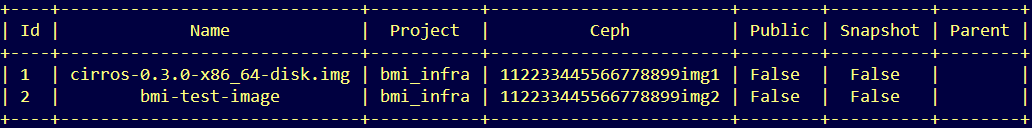
\includegraphics[scale=0.7]{figures/bmi-import-db-ls.png}
\end{center}
\caption{The output of running: \code{bmi db ls}}
%\label{fig:example_figure}
\end{figure}

The same thing can be viewed through the following command: \\

\code{
\text{} \\
\text{}\hspace{6mm} \index{bmi ls}bmi ls bmi\_infra \\
}

This will result in the following output:

\begin{figure}[!h] % Example of including images
\label{fig:bmi-workflow}
\begin{center}
%\includegraphics[width=0.5\linewidth]{#1}
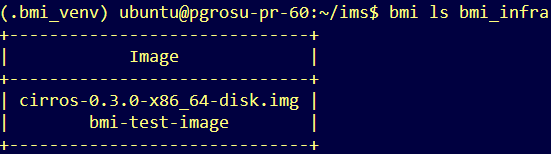
\includegraphics[scale=0.7]{figures/bmi-ls.png}
\end{center}
\caption{The output of running: \code{bmi ls}}
\end{figure}


Notice in Figure \ref{fig:ceph-imported-cloned-image} how in Ceph there now is a cloned image created with the name \code{112233445566778899img2}, since the golden image named \code{bmi-test-image} must be preserved.



\begin{figure}[!h] % Example of including images
\begin{center}
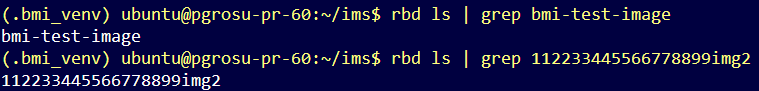
\includegraphics[scale=0.7]{figures/rbd-ls-bmi-test-image.png}
\end{center}
\caption{The seeing the images in Ceph}
%\label{fig:example_figure}
\label{fig:ceph-imported-cloned-image}
\end{figure}


\pagebreak

\subsection{Provisioning a Node Using BMI}

To \index{provision}provision a node in BMI, type the following command: 


\code{
\text{} \\
\text{}\hspace{6mm} \index{bmi pro}bmi pro bmi\_infra bmi\_node bmi-test-image bmi\_network bmi\_port \\
}

If the above processes successfully, you should see \code{Success} printed on your terminal screen, as follows: \\

\begin{figure}[!h] % Example of including images
\label{fig:bmi-workflow}
\begin{center}
%\includegraphics[width=0.5\linewidth]{#1}
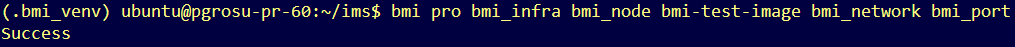
\includegraphics[scale=0.7]{figures/bmi-provisioning.png}
\end{center}
\caption{The output of running BMI provisioning command}
%\label{fig:example_figure}
\end{figure}

To see the new snapshot in BMI, run \index{bmi db ls}\code{bmi db ls} and you should see the following: \\

\begin{figure}[!h] % Example of including images
\label{fig:bmi-workflow}
\begin{center}
%\includegraphics[width=0.5\linewidth]{#1}
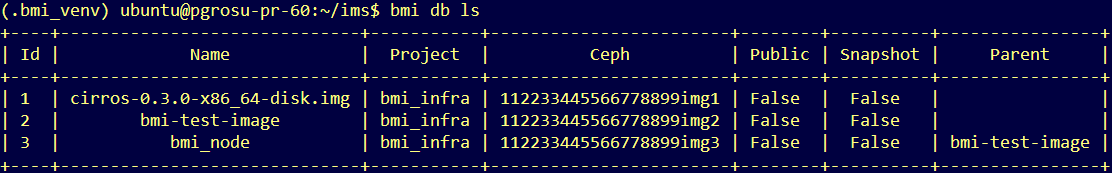
\includegraphics[scale=0.7]{figures/bmi-provisioning-db-ls.png}
\end{center}
\caption{Listing the newly provisioning in BMI}
%\label{fig:example_figure}
\end{figure}

%\pagebreak

Notice how the name is the node name itself (\code{bmi\_node}) who's parent is \code{bmi-test-image} is listed, with the \code{Parent} column set to \code{bmi-test-image}.   \\


\subsection{Creating a Snapshot Using BMI}

Snapshots provide the ability to get an instance of a state of an image at a point-in-time.  These are just a read-only copy, which would require to be cloned and flattened\footnote{Flattening an image makes it independent from the parent snapshot by copying the data to the child image.} in order to be writeable.   Snapshots in fact are central to protecting a golden image on Ceph, so that the original is preserved. \\

\pagebreak

To create a \index{snapshot}snapshot of a node in BMI, first make sure that the \underline{node is powered off}, and then type the following command: 

\code{
\text{} \\
\text{}\hspace{6mm} \index{bmi snap create}bmi snap create bmi\_infra bmi\_node bmi-test-image-snapshot \\
}

%\pagebreak

If the above processes successfully, you should see \code{Success} printed on your terminal screen, as follows: \\


\begin{figure}[!h] % Example of including images
\label{fig:bmi-workflow}
\begin{center}
%\includegraphics[width=0.5\linewidth]{#1}
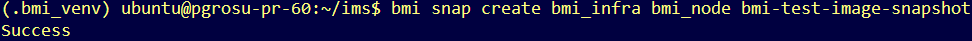
\includegraphics[scale=0.7]{figures/bmi-snapshot-create.png}
\end{center}
\caption{The output of creating a snapshot using BMI}
%\label{fig:example_figure}
\end{figure}



To see the new snapshot in BMI, run \index{bmi db ls}\code{bmi db ls} and you should see the following: \\

%\pagebreak

\begin{figure}[!h] % Example of including images
\label{fig:bmi-workflow}
\begin{center}
%\includegraphics[width=0.5\linewidth]{#1}
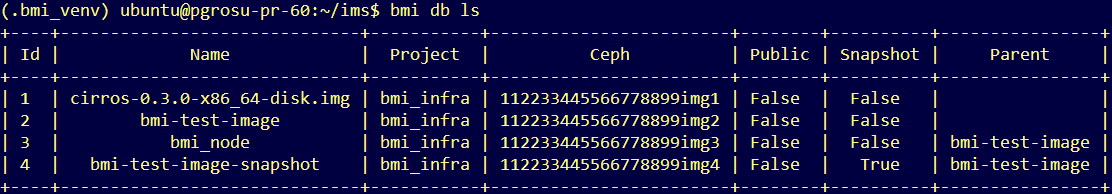
\includegraphics[scale=0.7]{figures/bmi-snapshot-db-ls.png}
\end{center}
\caption{Listing the newly created snapshot in BMI}
%\label{fig:example_figure}
\end{figure}


Notice how the \code{Snapshot} column is now set to \code{True}, with the \code{Parent} column set to \code{bmi-test-image}. \\  

%\pagebreak 

To see what is stored in Ceph, below is the output of running \code{rbd ls -l}: \\

\begin{figure}[!h] % Example of including images
\label{fig:bmi-workflow}
\begin{center}
%\includegraphics[width=0.5\linewidth]{#1}
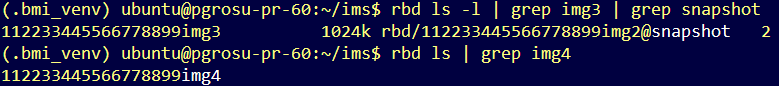
\includegraphics[scale=0.7]{figures/rbd-ls-snapshot.png}
\end{center}
\caption{The stored files in Ceph.}
%\label{fig:example_figure}
\end{figure}



\subsection{Deprovisioning a Node Using BMI}

To \index{deprovision}deprovision a node in BMI, type the following command: 

% bmi import bmi_infra bmi-test-image

\code{
\text{} \\
\text{}\hspace{6mm} \index{bmi dpro}bmi dpro bmi\_infra bmi\_node bmi\_network bmi\_port \\
}

If the above processes successfully, you should see \code{Success} printed on your terminal screen, as follows: \\


\begin{figure}[!h] % Example of including images
\label{fig:bmi-workflow}
\begin{center}
%\includegraphics[width=0.5\linewidth]{#1}
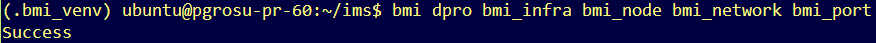
\includegraphics[scale=0.7]{figures/bmi-deprovisioning.png}
\end{center}
\caption{The output of running BMI deprovisioning command}
%\label{fig:example_figure}
\end{figure}

%\pagebreak

To see how BMI is updated, run \index{bmi db ls}\code{bmi db ls} and you should see the following: \\

\begin{figure}[!h] % Example of including images
\label{fig:bmi-workflow}
\begin{center}
%\includegraphics[width=0.5\linewidth]{#1}
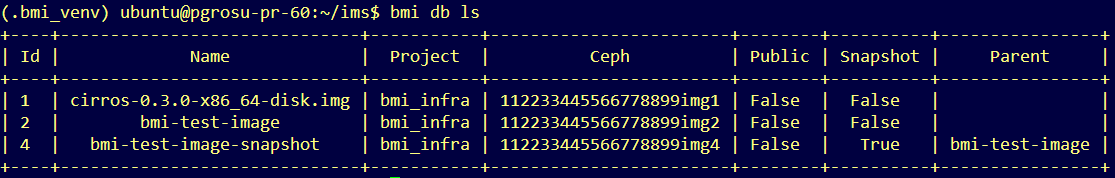
\includegraphics[scale=0.7]{figures/bmi-deprovisioning-db-ls.png}
\end{center}
\caption{Listing the newly created snapshot in BMI}
%\label{fig:example_figure}
\end{figure}




\subsection{Removing a Snapshot Using BMI}

To \index{remove a snapshot}remove a snapshot of a node in BMI, type the following command: 

\code{
\text{} \\
\text{}\hspace{6mm} \index{bmi snap rm}bmi snap rm bmi\_infra bmi-test-image-snapshot \\
}

%\pagebreak

If the above processes successfully, you should see \code{Success} printed on your terminal screen, as follows: \\

%\pagebreak


\begin{figure}[!h] % Example of including images
\label{fig:bmi-workflow}
\begin{center}
%\includegraphics[width=0.5\linewidth]{#1}
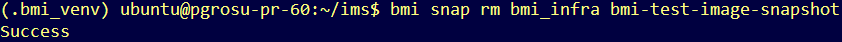
\includegraphics[scale=0.7]{figures/bmi-snapshot-remove.png}
\end{center}
\caption{The output of removing a snapshot using BMI}
%\label{fig:example_figure}
\end{figure}

To see that the \index{snapshot}snapshot was removed in BMI, run \index{bmi db ls}\code{bmi db ls} and you should see the following: \\

\begin{figure}[!h] % Example of including images
\label{fig:bmi-workflow}
\begin{center}
%\includegraphics[width=0.5\linewidth]{#1}
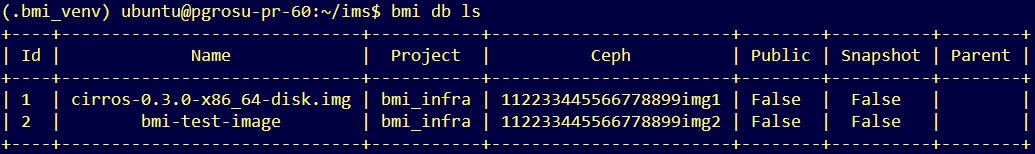
\includegraphics[scale=0.7]{figures/bmi-snapshot-remove-db-ls.png}
\end{center}
\caption{Showing that the snapshot was removed in BMI}
%\label{fig:example_figure}
\end{figure}

%\pagebreak 

To see that the snapshot does not exist in Ceph, below is the output of running \\
\code{rbd ls -l}: \\

\begin{figure}[!h] % Example of including images
\label{fig:bmi-workflow}
\begin{center}
%\includegraphics[width=0.5\linewidth]{#1}
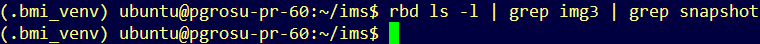
\includegraphics[scale=0.7]{figures/rbd-ls-snapshot-removed.png}
\end{center}
\caption{Showing that the snapshot does not exist in Ceph}
%\label{fig:example_figure}
\end{figure}



\subsection{Removing an Image Using BMI}

To \index{remove an image}remove an image in BMI, type the following command: 

\code{
\text{} \\
\text{}\hspace{6mm} \index{bmi rm}bmi rm bmi\_infra bmi-test-image \\
}

%\pagebreak

If the above processes successfully, you should see \code{Success} printed on your terminal screen, as follows: \\

%\pagebreak


\begin{figure}[!h] % Example of including images
\label{fig:bmi-workflow}
\begin{center}
%\includegraphics[width=0.5\linewidth]{#1}
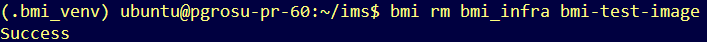
\includegraphics[scale=0.7]{figures/bmi-rm-db-ls.png}
\end{center}
\caption{The output of removing an image using BMI}
%\label{fig:example_figure}
\end{figure}

To see that the image was removed in BMI, run \index{bmi db ls}\code{bmi db ls} and you should see the following: \\

\begin{figure}[!h] % Example of including images
\label{fig:bmi-workflow}
\begin{center}
%\includegraphics[width=0.5\linewidth]{#1}
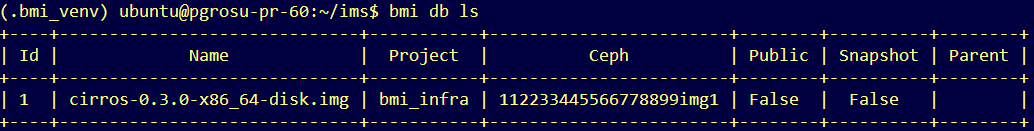
\includegraphics[scale=0.7]{figures/bmi-image-remove-db-ls.png}
\end{center}
\caption{Showing that the image was removed in BMI}
%\label{fig:example_figure}
\end{figure}


%\pagebreak 

To remove the image from Ceph, just type the following command:

\code{
\text{} \\
\text{}\hspace{6mm} \index{rbd rm}rbd rm bmi-test-image \\
}
 
You should now see that the image does not exist in Ceph, below is the output of running \\
\index{rbd ls}\code{rbd ls}: \\

\begin{figure}[!h] % Example of including images
\label{fig:bmi-workflow}
\begin{center}
%\includegraphics[width=0.5\linewidth]{#1}
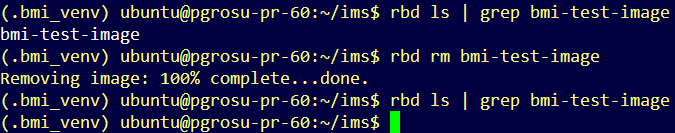
\includegraphics[scale=0.7]{figures/rbd-rm-bmi-test-image.png}
\end{center}
\caption{Showing that the image does not exist in Ceph}
%\label{fig:example_figure}
\end{figure}

\section{Existing the Virtual Environment}

To exit \index{virtualenv}\code{virtualenv}, type the following command: 

\code{
\text{} \\
\text{}\hspace{6mm} deactivate \\
}

%\pagebreak

Your terminal prompt should change to the following after typing the command: \\

\begin{figure}[!h] % Example of including images
\label{fig:bmi-workflow}
\begin{center}
%\includegraphics[width=0.5\linewidth]{#1}
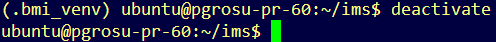
\includegraphics[scale=0.7]{figures/virtualenv-exit.png}
\end{center}
\caption{Existing the Virtual Environment \code{virtualenv}}
%\label{fig:example_figure}
\end{figure}


This completes the end-to-end training for learning how to use the most common BMI commands.

